\documentclass[twocolumn]{article}

%\usepackage[iso]{umlaute}
%\usepackage{german}
\usepackage{breakurl}
\usepackage{graphicx}
\setlength{\parindent}{0.3cm}
\setlength{\parskip}{1ex}
\setlength{\columnsep}{25pt}

\textwidth=17cm
\textheight=23cm
\setlength{\unitlength}{0.5cm}
\setlength{\parindent}{0.0cm}
\setlength{\parskip}{1ex}
\raggedbottom
\sloppy
%\addtolength{\evensidemargin}{-5cm}
\addtolength{\oddsidemargin}{-1.5cm}
\addtolength{\topmargin}{-2cm}

\sloppy

% Your name
\author{Trung Nguyen\\ Technische Universit\"at M\"unchen}

\title{Seminar Cloud Computing \\
       {\bf From Concept to Production: Enablement of TinyML in Industrial Setting}
}

% Date of your talk
\date{November 2024}

\usepackage{hyperref}

\begin{document}

\maketitle

\begin{abstract}
In recent years, Artificial Intelligence (AI) and Machine Learning (ML) have received tremendous amount of attention in both industry and research world. However, conventional Machine Learning demands high computing capability which limits its usage to only larger computing units. The paradigm shift to Tiny Machine Learning (TinyML) is revolutionizing industries by enabling the deployment of machine learning models on low-power, resource-constrained devices. Being one of the most rapid developing field of Machine Learning, TinyML promises to benefit multiple industries. However, building a production-ready TinyML system poses different unique challenges. In this paper, we explore the key obstacles faced when developing and deploying TinyML models in production environments, including model optimization, hardware limitations, software integration, and maintaining performance in real-world conditions. Additionally, we present real-world use cases of TinyML in industrial settings, showcasing its transformative impact in predictive maintenance, agriculture, and healthcare monitoring. We also discuss practical approaches and strategies presented by recent researches \cite{ren_tinyol_2021} to overcome these challenges, providing insights into how TinyML systems can be successfully scaled and implemented in production.
\end{abstract}

% \section defines numbered parts of the paper with titles
% there also are \subsection and \subsubsection
\section{Introduction}
\label{introduction}


Traditional Machine Learning Models, especially Deep Learning Models typically require substantial amount of computing capability to operate effectively. These models are often trained on powerful Graphics Processing Units (GPUs) and produce large models ranging from tens or hundreds of gigabytes (GB) down to smaller models in the range of 10 to 100 megabytes (MB). However, the memory requirements during runtime for these models far exceed what microcontrollers (MCUs) can handle.
The paradigm shift to TinyML is driven by the prevailing number of Microcontroller Units (MCU) currently circulating in the industry. According to a recent report \cite{noauthor_microcontroller_nodate,grandviewresearch_research_2023}, as of 2021, around 31 billion MCUs were shipped worldwide annually. The MCU market size is projected to increase in upcoming years \cite{noauthor_microcontroller_nodate}. This creates a big incentive for researchers and industry players to put effort into developing the technology further.
TinyML aims to enable data processing or inferencing directly on embedded systems, particularly on Internet Of Things (IOT), instead of streaming to the cloud. TinyML models can operate on energy- and memory-constrained devices by minimizing communication with external servers, using optimized architecture designs, and employing compression techniques such as quantization and pruning. The advancement of TinyML has positively influenced multiple industries and sectors such as: industrial IOT \cite{ray_review_2022}, healthcare \cite{bhamare_chapter_2024}, agriculture \cite{tsoukas_tinyml-based_2022}, IOT in smart-city \cite{hussein_original_2024,ray_review_2022}. \\[0.25cm]

Although various organizations have been actively investing resources into machine learning and data science projects, only around 13\% of these projects successfully progress to production.\footnotemark \footnotetext{\url{https://venturebeat.com/ai/why-do-87-of-data-science-projects-never-make-it-into-production/}} 
This low success rate highlights the complex challenges and gaps in translating ML concepts into fully functional, production-grade systems, especially in the realm of TinyML. In this paper, we aim to address these challenges and outline what is necessary to transition a TinyML project from concept to production, ultimately creating value for industrial applications. In Chapter~\ref{tinyml_overview}, we provide an in-depth overview of the fundamental concepts, techniques, and development pipeline of TinyML. Following this, in Chapter~\ref{prod_tinyml}, we draw on recent research to investigate the specific challenges encountered in developing and deploying TinyML models in production environments, as well as practical strategies to overcome these obstacles. Next, in Chapter~\ref{use_cases}, we explore real-world applications of TinyML in industrial settings, illustrating its transformative potential. Finally, in Chapter~\ref{future_of_tinyml}, we consider the future trajectory of TinyML, discussing upcoming advancements and their implications for broader industrial adoption.
\begin{figure}
	\centerline{
	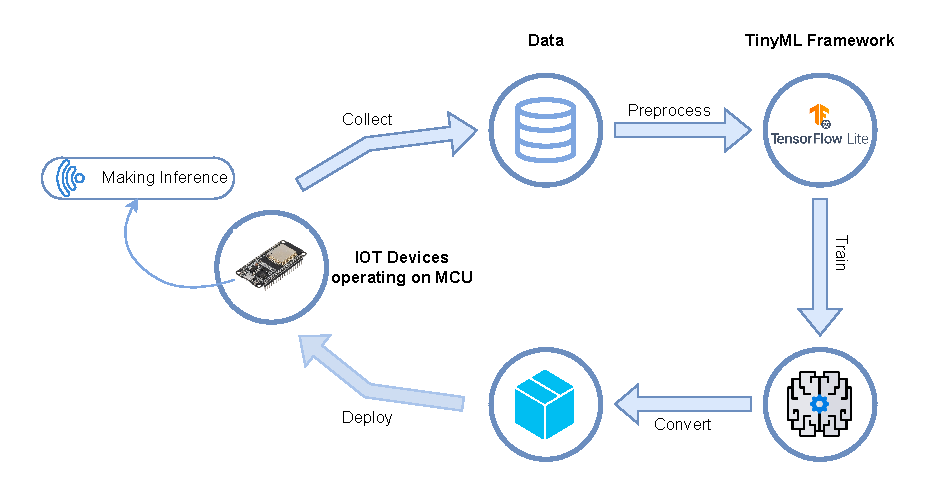
\includegraphics[width=1\columnwidth,height=0.23\textheight]{resource/tinyml_deployment.pdf}
	}
	\caption{TinyML Deployment pipeline (adapted from Ren et al. \cite{ren_tinyol_2021})}
	% A label to allow refering to this figure in the text.
	\label{TUM}
\end{figure}

\section{TinyML Overview} 
\label{tinyml_overview}

\subsection{Key Concepts and Techniques}

Pruning removes unnecessary neurons or connections from a neural network to reduce its size and complexity. This optimization lowers memory and computational demands, making the model faster and more efficient for deployment on resource-limited devices like microcontrollers.

Quantization reduces the precision of model parameters (e.g., from 32-bit to 8-bit), which decreases model size and computational needs. This technique enables efficient model inference on devices with limited memory and processing power, such as those used in TinyML applications.

With the TinyML model running on edge, the data is stored, processed and analyzed internally rather
than at an external server or cloud. 

\subsection{TinyML pipeline}



\paragraph{Data Collection:}
	The workflow starts with collecting data from an IoT device. This data serves as the input for training machine learning models. The IoT device can gather various types of data depending on the application, such as sensor data in smart homes or for environmental monitoring, IoT sensors may record temperature, humidity, and air quality data. In healthcare applications, devices like wearable fitness trackers collect medical signals to monitor heart rate or blood pressure, this aspect will be elaborated in later Use Cases ~\ref{use_cases} sections. This raw data serves as the foundation for training the machine learning model, ensuring it captures relevant real-world conditions. \\[0.10cm]

\paragraph{Preprocessing:}
	Once the data is collected, it undergoes preprocessing to clean and prepare it for model training. Tasks in this stage might include tasks such as normalization to adjust sensor readings to a common scale, handling missing values to fill gaps in environmental data using interpolation or removing incomplete data points, or feature extraction. These steps ensure the model receives high-quality input, improving training performance and generalization.\\[0.10cm]

\paragraph{Model Training:}
	The preprocessed data is then fed into an ML framework, where a machine learning model is trained. This stage involves using machine learning algorithms to find patterns in the data, building a predictive or analytical model that can generalize from the data. For example, in the renewable energy industry, a neural network might be trained to recognize defect from wind turbine from features extracted from relevant sensors. The model is trained to detect patterns and relationships in the data, creating a predictive system that generalizes to unseen inputs. \\[0.10cm]

\paragraph{Model Conversion:}
	Model conversion is the part when the ML model becomes tiny, hence TinyML. Once the model is trained, it is converted into a format suitable for deployment on resource-constrained devices, like microcontrollers. This step might involve techniques such as quantization (reducing the precision of model weights) or pruning (removing unnecessary parts of the model) to reduce the model’s size and computation needs. These techniques ensure the model fits within the memory and processing limits of edge devices.
	\\[0.10cm]

\paragraph{Model Packaging:}
	In this step, the converted model is packaged with all necessary runtime components to enable execution on the target device. This includes bundling the model with any necessary runtime components to allow it to be executed efficiently on the target device. For example, one can bundle a TensorFlow Lite model with inference libraries that allow it to run on microcontrollers like Raspberry Pi Pico. Packaging ensures the model is ready for deployment in a streamlined and executable format.
	\\[0.10cm]

\paragraph{Deployment:}
	The next step involves deploying the model onto an IoT device. This means transferring the model to the device, configuring it to run in the intended application and setting it up for real-time inference or operation in the field. For example, to deploy a fall-detection model on an Arduino Nano 33 BLE Sense, it means to upload the code and model to the Arduino via USB. Test the device with simulated falls, and once validated, it can run locally, detecting falls in real-time and triggering alerts.\\[0.10cm]


\paragraph{Inference:}
	Finally, the deployed model performs inference on the IoT device. Inference refers to the process of using the model to make predictions or decisions based on new data collected by the IoT device. The model operates locally on the device without needing continuous cloud connectivity, enabling real-time decision-making at the edge.\\[0.10cm]



\section{Enablement of TinyML in Industrial Setting}
\label{prod_tinyml}

\subsection{Challenges}

The fundamental pipeline for deploying a TinyML model to a microcontroller, as described above in Chapter~\ref{tinyml_overview}, provides a general framework for model development and deployment. However, in industrial settings, this pipeline often falls short due to a variety of challenges unique to production environments. Firstly, industrial applications typically demand more robust and adaptable systems, requiring continuous model updates and seamless integration within complex IoT infrastructures. Secondly, these demands introduce specific obstacles, such as the inability to regularly update models on resource-constrained devices and the difficulty of integrating TinyML systems with existing IoT architectures.

\subsubsection{Adaptation to unseen scenarios and constantly changing conditions}
In traditional machine learning (ML), models can be regularly updated with new data through a constant internet connection, allowing them to stay relevant as conditions evolve. This capability, however, is often unavailable for TinyML models deployed on microcontroller units (MCUs) in IoT or edge devices, which typically lack continuous internet access. Consequently, once a model is deployed on an MCU, it may remain static for extended periods, operating without the benefit of regular updates.\\[0.1cm]

This static deployment significantly impacts TinyML models over time, especially in dynamic environments where data patterns evolve. In real-world applications, conditions rarely remain constant, and the input data the model receives can change due to factors such as seasonal variations, environmental shifts, or user behavior changes. Without regular updates, a static model can struggle to adapt to these evolving patterns, a challenge known as concept drift (when the relationship between input and output changes) and data drift (when the distribution of input data changes). Both forms of drift can lead to a decline in model performance, making it essential to consider ways to address these challenges in TinyML deployments.


\subsubsection{Integrating with Existing IOT System and Management of TinyML Models in Heterogeneous Devices}
Integrating TinyML-enabled microcontrollers (MCUs) into existing IoT systems presents several unique challenges. IoT infrastructures are often built on established architectures, protocols, and data formats that may not be directly compatible with TinyML MCUs. Adapting these MCUs to work within the existing IoT ecosystem requires significant customization to ensure seamless data exchange, communication, and interoperability.\\[0.1cm]

Moreover, existing IoT systems frequently rely on centralized processing or cloud-based analytics, while TinyML emphasizes local computation on edge devices. This architectural shift introduces complexities in synchronizing data and managing hybrid workflows that combine cloud and edge processing. Industrial IoT deployments also come with strict security and compliance requirements, so integrating TinyML MCUs necessitates additional security protocols, device authentication, and data encryption to maintain data integrity across the IoT network.\\[0.1cm]

Maintenance and scalability issues can complicate the integration of TinyML into IoT systems at scale. Updating models on distributed MCUs, managing firmware compatibility, and monitoring device health require robust infrastructure and automated processes, adding layers of complexity to deploying and managing TinyML solutions within existing IoT frameworks. Moreover, to manage and operate such sophisticated system requires deep technical capability which many of professionals with good domain lacks. This urges not only the need for effective methods to manage and maintain TinyML systems at scale but also the importance of making these systems accessible to a broader range of professionals. Enabling more individuals to work with TinyML systems will be crucial for ensuring widespread adoption and operational success in industrial environments. \cite{hussein_original_2024, paul_rethinking_2021, de_prado_robustifying_2020,ren_synergy_2021,roshan_adaptive_2021}.\\[0.1cm]


\subsection{Bringing TinyML to production environment}

To address these challenges, recent research by Ren et al. \cite{ren_tinyol_2021, ren_how_2022, ren_device_2024} proposes innovative solutions, including advanced on-device learning techniques and frameworks for seamless TinyML integration with IoT systems. These approaches tackle hardware constraints, dynamic adaptation needs, and scaling complexities, paving the way for efficient and scalable TinyML deployments in industrial settings.

\subsubsection{Advanced On Device Learning Methods}
Creating a general ML model for general use is impractical for MCUs due to their resource-constraint nature. A simple ML model can easily exceed the hard storage room of a MCU. Moreover, for a general ML model to function, it needs to be updated with field data on the fly, which usually not possible as MCUs do not possess constant connection to the Internet, especially while operating at edge.\\[0.1cm]

In their paper on TinyOL (Tiny Machine Learning with Online Learning), Ren et al. introduced a novel system that enables on-device learning. This approach allows models deployed on embedded devices, such as sensors or microcontrollers, to learn and adapt in real time without requiring external retraining.

\begin{figure}
	\centerline{
	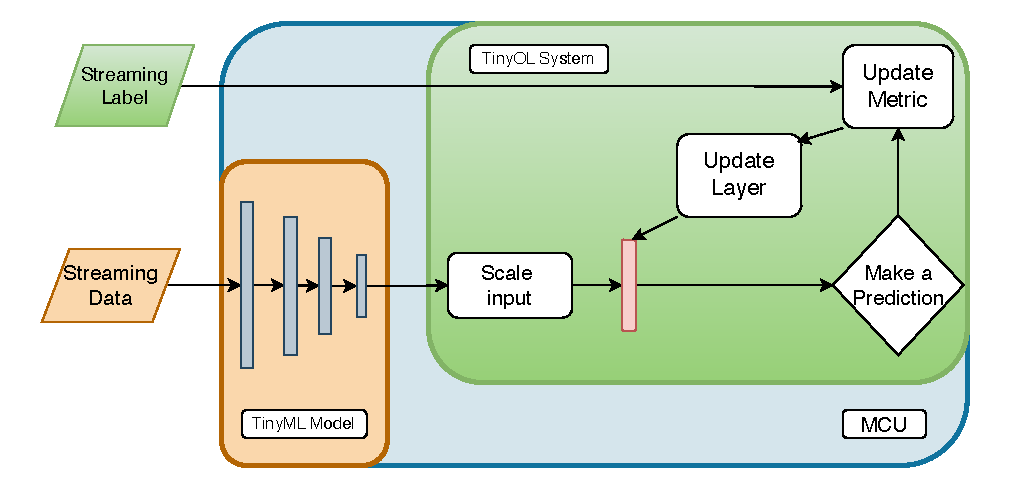
\includegraphics[width=1\columnwidth,height=0.2\textheight]{resource/tinyol_on_mcu.pdf}
	}
	\caption{TinyOL Components on MCUs (adapted from Ren et al. \cite{ren_tinyol_2021})}
	\label{TinyOL}
\end{figure}

The core of TinyOL lies in the additional layer marked in red in Figure~\ref{TinyOL} referred to as the \textbf{update layer} which consists of neurons that can be customized, initialized, and updated on the fly. This layer serves as an output layer that can adapt to new data while preserving the original network's structure. Following is the breakdown of the other components in Figure~\ref{TinyOL}.

\begin{itemize}
    \item \textbf{Streaming Data}:
    This component represents the live data input collected by the MCU from its environment. It is fed into the TinyML model continuously, allowing the system to make predictions based on real-time information.

    \item \textbf{TinyML Model}:
    The core machine learning model deployed on the MCU. It takes streaming data as input and performs initial processing. This model consists of several layers (depicted by vertical bars), which extract features from the data.

    \item \textbf{Scale Input}:
    After the TinyML model processes the input data, it passes through a scaling component. This step standardizes or normalizes the data to ensure it fits the model’s expected input distribution, helping maintain consistent performance as new data arrives.

    \item \textbf{Make a Prediction}:
    After scaling and processing, the TinyOL system uses the model to make predictions. This decision node represents the point at which the system outputs a result based on the latest input data.

    \item \textbf{Update Metric}:
    When true labels (ground truth) are available, the system can update evaluation metrics based on the prediction’s accuracy. This component helps measure model performance and provides feedback for updating the model’s parameters.

    \item \textbf{Streaming Label}:
    This component represents the true labels or ground truth data available intermittently. When available, it is used to calculate metrics and adjust the update layer, enabling the model to correct itself over time and adapt to changing data patterns.
\end{itemize}


\paragraph{TinyOL Workflow}
The TinyOL workflow, as outlined by the authors’ algorithm \cite{ren_tinyol_2021}, consists of the following steps:
\begin{enumerate}
    \item \textit{Initialization:} TinyOL initializes both the TinyML model and the TinyOL system for on-device learning.
    \item \textit{Streaming Data Processing:} As new data points are received from the data stream, TinyOL processes each sample iteratively.
    \item \textit{Normalization and Standardization:} TinyOL continuously updates the running mean and variance of the incoming data to standardize it, ensuring compatibility with the model’s input requirements.
    \item \textit{Prediction and Model Update:} TinyOL uses the standardized input to make a prediction. If a true label is available, TinyOL computes the error between the prediction and the label, updating evaluation metrics. The model’s weights are then adjusted accordingly using techniques such as \textbf{stochastic gradient descent (SGD)}.
\end{enumerate}

\paragraph{Minium Resource Consumption:}
After processing each data point, TinyOL discards it to conserve memory. Compared to traditional batch/offline training methods, this efficient approach enables TinyOL to handle high volumes of streaming data, which is essential for resource-constrained MCUs with limited storage and processing capacity. The framework operates with as little as 7 KB of RAM and 135 KB of Flash memory.

\paragraph{Continuous Adaptation:}
TinyOL’s architecture allows it to continuously adapt to new data patterns over time, addressing issues like \textbf{concept drift} and \textbf{data drift}. By updating model weights in real time, the system ensures that the deployed model remains relevant and can handle changes in input data characteristics that may not have been present during initial training.

\subsubsection{Management of TinyML systems at scale}

There has been increased attention to TinyML Management with different methods proposed such as: TinyML as a service , Model Card to describe and organize the information of trained models \cite{mitchell_model_2019}, or TinyML Operations (TinyMLOps) \cite{antonini_tiny-mlops_2022} to build an abstraction layer for various hardware compilers. However, these approaches reveal certain drawbacks as they lack features for users to store and exchange information about existing resources. \\[0.1cm]

The paper introduces a TinyML low-code management framework called SeLoC-ML (Semantic Low-Code ML), designed to simplify the deployment, management, and scaling of TinyML applications. The essentials of SeLoC-ML can be broken down into two main parts: to build a KG ontology on the existing overall TinyML system and to inject the KG into a low-code platform \footnote{A low-code platform is a development environment that enables application creation through visual interfaces and minimal coding, making it accessible to users with limited programming knowledge. \url{https://www.ibm.com/topics/low-code/}}. 


\begin{figure*}[t]
	\centerline{
	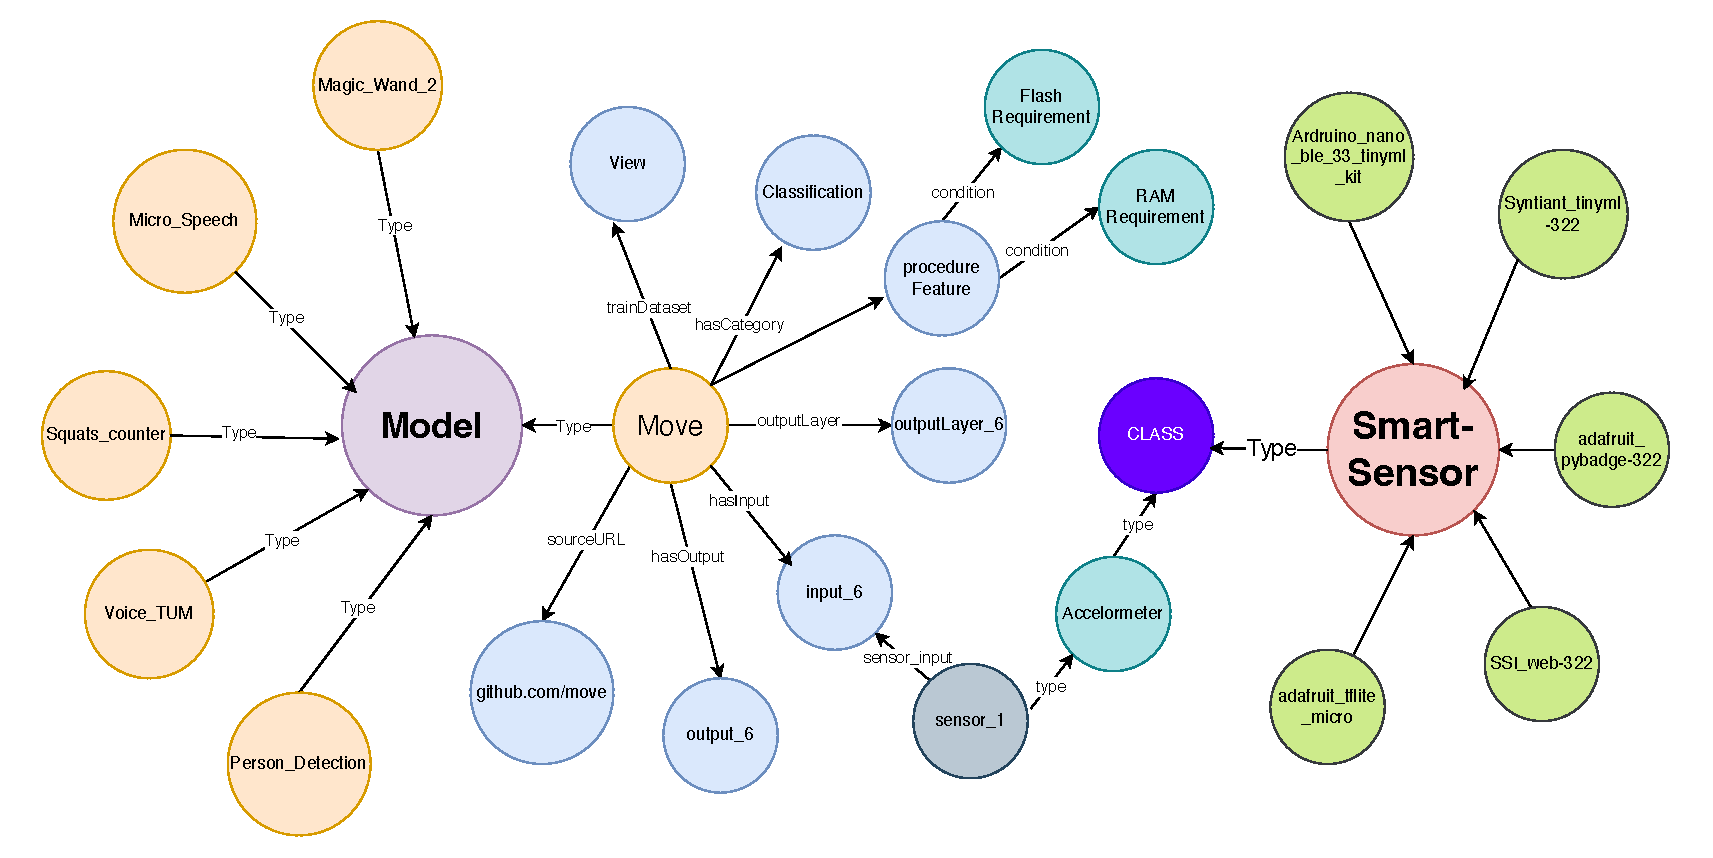
\includegraphics[width=0.9\textwidth,height=0.4\textheight ]{resource/KG.pdf}
	}
	\caption{Visualization of System's Knowledge Graph (Simplified) adapted from \cite{ren_tinyol_2021}}
	\label{KG}
\end{figure*}


\paragraph{Contruction of the Knowledge Graph (KG):} 

By reusing existing standards, like the \textbf{Semantic Sensor Network(SSN)} and \textbf{W3C Thing Description (TD)}  \footnote{\url{https://www.w3.org/WoT/}}
ontologies (a structured schema), an ontology that includes definitions and metadata for TinyML models, such as neural network architecture, layer configurations, and hardware requirements can be built. These data then can be stored using a graph database to facilitate management, discovery, and deployment of TinyML applications.\\[0.1cm]

Figure \ref{KG} is a simplified visual example of a knowledge graph. A total of 6 ML models are shown on the left side of the figure. One model is especially displayed in details. The "Move" model, as depicted in the knowledge graph, represents a TinyML motion-detection or activity-recognition model with defined input and output requirements, metrics, and compatibility conditions. By including this model in the knowledge graph, the TinyML management system can ensure the Move model is deployed on compatible hardware, facilitating real-time motion analysis or gesture detection in various applications. On the right-side cluster represents various IoT devices or sensor types, each represented by green nodes labeled with device names like “arduino\_nano\_ble\_33” and “adafruit\_tflite\_micro.” Finally, the link from Smart Sensor to Move Model in the knowledge graph represents a data dependency and compatibility relationship. It indicates that for the Move Model to function effectively, it requires input from a device that fits the description of a Smart Sensor.\\[0.1cm]

\paragraph{Integrating into a low-code platform:}
Having the knowledge graph in form of a graphDB constructed, next step is to integrate with a low-code platform, to enable non-experts to manage and deploy TinyML models across diverse embedded devices. There are several low-code platforms in the market such as: SAP Build \footnote{\url{https://www.sap.com/products/technology-platform/build.html}} or Siemens Mendix \footnote{\url{https://www.mendix.com}}. Low-code software development cuts down on coding by using simple, drag-and-drop visual tools. This makes it quick to build, easy to update, and straightforward to manage business applications without needing much programming experience.\\[0.1cm]



This approach addresses the challenges of \textbf{updating models on distributed MCUs} and \textbf{managing firmware compatibility} by leveraging Semantic Web technologies and a Knowledge Graph (KG) to centralize and standardize information about TinyML models and IoT devices. The framework’s \textit{ontology} provides a standardized way to describe ML models and IoT devices, facilitating tracking of model versions, configurations, and updates across various devices. By storing information about model updates, dependencies, and compatibility requirements in the KG, the system enables automated discovery of compatible models for each device, allowing administrators to push updates more efficiently. The \textit{querying capabilities} of the Knowledge Graph make it easy to identify which MCUs require updates, simplifying model deployment across large-scale, distributed systems. Additionally, the KG maintains details about each device’s firmware, hardware specifications, and compatibility requirements, ensuring that only compatible firmware and model updates are deployed. This centralized approach minimizes the risk of deploying incompatible firmware or models, which is crucial in environments with diverse MCU configurations. 


\section{Use Cases of TinyML in Industrial Setting}
\label{use_cases}

\subsection{Industrial Predictive Maintenance}

Predictive Maintenance (PdM) refers to a practice where business, based on series of historical and failure data, to predict in the future potential health and availability of equipments as well as anticipate defects in advance before they occur, thereby increase equipment lifespan, reduce downtime and operating cost \cite{ooko_application_2024}. The practice of constantly observing and predicting has its own inherent flaws and challenges such as financial and organizational constraints, limited source of historical data, and deployment of suitable PdM model \cite{zonta_predictive_2020}. \\[0.1cm]

TinyML offers a promising solution to several challenges by enabling intelligent predictive maintenance through embedded, low-power machine learning algorithms that can process data directly on the device. Unlike traditional ML in PdM, which typically relies on centralized data centers and cloud infrastructure, TinyML method helps close the gap in deploying predictive maintenance models by reduce the dependence on large-scale data infrastructure and addressing data source and computational limitations \cite{abadade_comprehensive_2023}. By allowing edge devices to process and analyze data locally, TinyML reduces the need for extensive data transmission and storage \cite{ooko_tinyml_2021}. This enhances the efficiency and reliability of IoT systems by ensuring that only relevant, actionable insights are sent back to the central system.

\subsubsection{TinyML vs. Standard ML}

According to \cite{achouch_predictive_2022,zonta_predictive_2020}, there are 80\% solutions for PdM found in literatures are ML-based and only 20\% are TinyML-based. This shows that the TinyML-based solutions in industry are still under-discovered as it still has certain weaknesses compared to standard ML approaches.\\[0.1cm]

Standard ML models operation requires a lot more computational power, however, as result, are able to handle complex situations at higher accuracy. On the other hand, Standard ML performs with high latency and power consumption, due to the need to transmit data to servers which poses security breaches. At the edge, where electricity and network connectivity are limited, TinyML proves to be a more viable solution for PdM tasks. 

\subsubsection{Use Cases in PdM}

\paragraph{Anomaly Detection}

In extreme environments such as at the ocean where thousands of wind turbines are deployed, TinyML has been applied to detect misbehavior and early signs defections in turbines by analyzing turbines' spin behaviors. First, a study shows that novel sensors such as the ISM330IS Inertial Measurement Unit (IMU) from STMicroelectronics enables an onboard Intelligent Sensor Processing Unit (ISPU) that allows some data processing to be computed on-board. In combination with Infrared thermographic and continuous line laser thermographic techniques to visualize damage in wind turbines, TinyML models can provide real-time analysis and defect detection at the edge without extensive data transmission \cite{rabbi_novel_nodate}. \\[0.1cm]

Another study showcased a system designed to detect anomalies in submersible pumps at wastewater plants. This system leverages an ESP32DEVKIT microcontroller paired with temperature and vibration sensors. By employing an Isolation Forest model for edge-based anomaly detection, the study highlights the feasibility of retrofitting existing equipment with TinyML capabilities.\cite{antonini_tinyml_2022}\\[0.1cm]

In a research that deploys a TinyML model on ESP-WROOM-32 MCU, thermal images of machinery can also be analyzed. Inferred data is then sent via MQTT only upon detection of anomalies to enhance maintenance efficiency. \cite{oliveira_edge_2022}

\paragraph{Operational Monitoring and Analysis}

In extreme environments, continuous monitoring of machinery operations becomes increasingly critical, as maintenance and repair costs tend to escalate over time. TinyML enables continuous monitor for operational efficiency, safety, or specific conditions indicative of the need for interventions.\cite{aemt_navigating_nodate}\\[0.1cm]

A study has been demonstrated for real-time impact localization on thin plastic plates using low-power, resource-constrained IoT devices. This approach leverages data from piezoelectric sensors and employs machine learning models, specifically Random Forest and Shallow Neural Networks, to analyze impact locations. The implementation runs efficiently on an Arduino NANO 33 BLE microcontroller, showcasing the feasibility of deploying such systems on embedded devices. \cite{noauthor_smart_nodate}.\\[0.1cm]


Another use case involves an ultralow-power Smart IoT device designed to monitor the activity of handheld power tools in construction environments. Utilizing TinyML for edge processing, the system categorizes tool usage into various operational modes, including transport, no-load, metal drilling, and wood drilling. This categorization enables optimized maintenance, extended tool lifecycles, and enhanced safety measures. The device features temperature, humidity, and acceleration sensors for data collection and employs Bluetooth Low Energy (BLE) and Near Field Communication (NFC) technologies for efficient communication and activation. \cite{giordano_design_2022}


\subsection{Smart Agriculture}
Other sector that TinyML has the most influence on is Agriculture.  By enabling real-time, on-device data processing and decision-making, TinyML is empowering farmers to optimize resource usage, increase productivity, and promote sustainable farming practices. As the technology continues to evolve, we can expect to see even more innovative applications of TinyML in agriculture, contributing to global food security and environmental sustainability.


\paragraph{Precision Agriculture}
A recent study explores the integration of Tiny Machine Learning (TinyML) with Unmanned Aerial Vehicles (UAVs) for precision agriculture applications. Using the Edge Impulse framework and ESP EYE 32, the study optimizes key parameters to minimize resource use while maintaining accuracy. Experiments highlight the effectiveness of single-labeled data for disease classification, achieving 91.67\% testing accuracy in binary classification. This work demonstrates the transformative potential of TinyML-powered UAVs in agriculture, making the way for intelligent, resource-efficient systems. \cite{annadata_tinyml_2024}


\paragraph{Crop, Soil Monitoring and Automated Farming Operations}

Another research proposes a power- and delay-aware TinyML model optimized for agricultural soil quality monitoring \cite{bhattacharya_deploying_2024}. After applying advanced techniques Dynamic Voltage and Frequency Scaling (DVFS), Sleep/Wake Strategies, Energy Harvesting, and Task Partitioning, the model achieves an 8.5\% reduction in energy consumption and a 10.4\% decrease in delay while maintaining high accuracy. The model enables real-time monitoring of soil parameters like moisture, pH, and nutrients using low-power microcontrollers, providing timely insights for improved soil management. The system can be trained to initiate watering based on specific environmental conditions, ensuring efficient water use and reducing waste. This approach extends device battery life, reduces environmental impact, and supports sustainable, resource-efficient agriculture. \\[0.1cm]

Furthermore, another paper presents a smart agriculture system based on TinyML. By integrating cameras with TinyML models, early detection of crop diseases and pest infestations becomes possible, allowing for timely interventions. \cite{tsoukas_tinyml-based_2023}. The integration of TinyML with embedded systems leads to cost savings by optimizing resource usage, reducing manual labor, and minimizing waste. This contributes to more economically viable farming practices.



\subsection{Healthcare Monitoring}

Besides disrupting smart agriculture, the integration of TinyML into healthcare is transforming how medical data is collected, processed, and analyzed, particularly in remote and resource-constrained environments. By enabling real-time analysis directly on low-power devices, TinyML is revolutionizing patient monitoring and diagnostics, offering solutions that are not only efficient but also scalable. From wearable devices tracking vital signs to portable systems detecting critical health conditions, TinyML is reshaping the future of personalized healthcare. Below, we explore specific use cases where TinyML is making significant strides in healthcare monitoring.\\[0.1cm]

A recent paper presents a TinyML-based cardiac monitoring device for real-time detection of cardiac signals using ECG and PPG waveforms. Built with low-cost sensors (Sparkfun AD8232 and MAX30102) and an Arduino Nano 33 BLE microcontroller, the device processes signals efficiently at the edge. The system achieves high accuracy, with 98.8\% for ECG and 100\% for PPG, while minimizing energy consumption through optimized, quantized models. By enabling rapid analysis and reliable metrics like Heart Rate Variability (HRV) and stress levels, the device demonstrates its potential for accessible, real-time healthcare, especially in remote or resource-constrained environments.\cite{r_tiny_2024}\\[0.1cm]


The TinyML-based system presented in another paper is used for continuous blood pressure (BP) estimation through real-time processing of photoplethysmogram (PPG) signals, which are optical signals generated by measuring changes in blood volume in tissues using a light source and a photodetector. This approach eliminates the need for traditional cuff-based BP monitors, offering a non-invasive and more convenient alternative for long-term monitoring. The system is highly effective, achieving compliance with medical standards such as the Association for the Advancement of Medical Instrumentation (AAMI) and the British Hypertension Society (BHS). These standards ensure that the device meets the required accuracy and reliability benchmarks. Additionally, the system’s edge-based design enhances privacy, reduces latency, and enables use in environments with limited or no internet connectivity, making it particularly suitable for remote healthcare settings. \cite{sun_case_2023}\\[0.1cm]


TinyML is transforming healthcare by enabling real-time, on-device analysis for patient monitoring and diagnostics, particularly in remote and resource-constrained settings. From cardiac monitoring devices with high accuracy to non-invasive blood pressure estimation systems compliant with medical standards, TinyML enhances accessibility, privacy, and efficiency. These advancements demonstrate TinyML’s potential to revolutionize personalized healthcare through affordable and scalable solutions.


\section{Future of TinyML}
\label{future_of_tinyml}

The future of TinyML holds immense potential as it continues to evolve to meet the demands of diverse industrial applications. Key trends that are expected to drive TinyML's progress include advancements in model optimization techniques, integration with edge AI, and improvements in hardware capabilities. Enhanced techniques like federated learning for TinyML could allow devices to learn collaboratively without sharing raw data, addressing both data privacy and adaptability in dynamic environments. Additionally, further development in quantization, pruning, and neural architecture search will allow models to be more efficiently deployed on constrained devices, expanding TinyML’s applicability.\\[0.1cm]

The expansion of 5G and the evolution of connectivity standards may also accelerate TinyML adoption, as these advancements could support more reliable intermittent connectivity for edge devices. This would facilitate more frequent model updates and allow TinyML models to synchronize with central systems when needed, even in remote areas. Another future direction is the integration of TinyML with the Internet of Things (IoT) on a larger scale, making real-time analytics accessible across widespread networks of low-power devices. TinyML is also expected to expand in areas like smart cities, environmental monitoring, and autonomous systems, where real-time data processing on edge devices is crucial. As the ecosystem grows, more low-code platforms and management frameworks, such as SeLoC-ML, will likely emerge, empowering a broader range of professionals to develop, deploy, and maintain TinyML systems effectively.\\[0.1cm]


Furthermore, addressing challenges like environmental sustainability, ethical considerations, and device disposability will be crucial to ensuring responsible growth. With increasing research, specialized datasets, and educational resources, TinyML continues to thrive as a transformative technology, fostering innovation while making machine learning more accessible, efficient, and impactful.\cite{prakash_tinyml_2024}


\section{Conclusion}
\label{conclusion}

TinyML represents a paradigm shift in the field of machine learning, allowing for the deployment of intelligent systems on resource-constrained devices. By enabling real-time data processing and inference at the edge, TinyML addresses many limitations of traditional machine learning, including high power consumption, dependency on cloud infrastructure, and latency issues. This paper has explored the multifaceted challenges of transitioning TinyML systems from concept to production, including hardware constraints, the need for adaptable models, and the intricacies of integrating TinyML into existing IoT frameworks. Through innovative approaches like TinyOL for on-device learning and SeLoC-ML for low-code management, the challenges of scalability, adaptability, and efficient system management are being addressed effectively.\\[0.1cm]

The practical applications of TinyML discussed in this paper underscore its transformative potential across a variety of industrial sectors. In predictive maintenance, TinyML provides on-device analytics to detect anomalies and optimize machinery performance in real-time. In agriculture, it empowers farmers with precision tools for monitoring soil quality, crop health, and environmental conditions, driving sustainable farming practices. Similarly, healthcare monitoring applications demonstrate how TinyML improves accessibility and efficiency through devices capable of continuous health monitoring, such as cardiac and blood pressure monitoring systems.\\[0.1cm]

As TinyML continues to evolve, its potential for widespread adoption in industrial settings is becoming increasingly evident. Advances in hardware efficiency, federated learning, and low-code platforms promise to make TinyML more accessible to non-experts while addressing scalability and operational challenges. Moreover, the integration of TinyML with cutting-edge technologies like 5G, IoT, and edge AI paves the way for smarter systems capable of handling diverse applications, from environmental monitoring to autonomous systems.\\[0.1cm]

Looking ahead, TinyML must address challenges related to sustainability, device lifecycle management, and ethical considerations. Efforts to reduce e-waste, enhance energy efficiency, and maintain data privacy will be critical for responsible growth. With robust research, technological advancements, and a growing community of practitioners, TinyML is poised to shape the future of intelligent computing, driving innovation and efficiency across industries while making machine learning more inclusive and impactful.


\bibliographystyle{plain}
% Literature sources are to be found in seminarpaper.bib
\bibliography{seminarpaper}
\end{document}
